\def \Subject {گام چهارم: مقایسه با سایر پروتکل های بی سیم}
\section{\Subject}
پس از جمع آوری اطلاعات کامل راجع به Zigbee و فهمیدن آن به طور کامل آن را با دیگر پروتکل های بیسیم مقایسه می کنیم.
در واقع حال که به طور کامل با این پروتکل آشنا شدیم می توانیم آن را با دیگر پروتکل های بی سیم مقایسه کنیم.
پروتکل و تکنولوژی های زیادی وجود دارند که برای ارتباطات بی سیم استفاده می شوند.
این پروتکل ها برای ارتباطات مختلفی مورد استفاده قرار می گیرند.
مثلا پروتکل هایی برای ارتباطات کوتاه مدت و پروتکل هایی برای ارتباطات بلند مدت وجود دارند.
همچنین پروتکل هایی برای ارتباطات کوتاه مدت در فاصله های کوتاه و پروتکل هایی برای ارتباطات کوتاه مدت در فاصله های بلند وجود دارند.
و پروتکل هایی برای ارتباطات بلند مدت در فاصله های کوتاه و پروتکل هایی برای ارتباطات بلند مدت در فاصله های بلند وجود دارند.
حال با توجه به جستجوی هایی که انجام دادم و تحقیقاتی که کردم ،
در این بخش به مقایسه آن با پروتکل های بی سیم دیگر با Zigbee می پردازیم:

\subsection{تعریفی اجمالی از پروتکل های بی سیم دیگر}

\begin{itemize}

    \item 
    {
        \textbf{Bluetooth} :
        بلوتوث یک استاندارد فناوری بی سیم کوتاه برد است که برای تبادل داده بین دستگاه های ثابت و موبایل در فواصل کوتاه و ایجاد شبکه های شخصی استفاده می شود. در پرکاربردترین حالت، توان انتقال به 2.5 میلی وات محدود می شود که برد بسیار کوتاهی تا 10 متر را به آن می دهد.
        \begin{figure}[H]
            \centering
            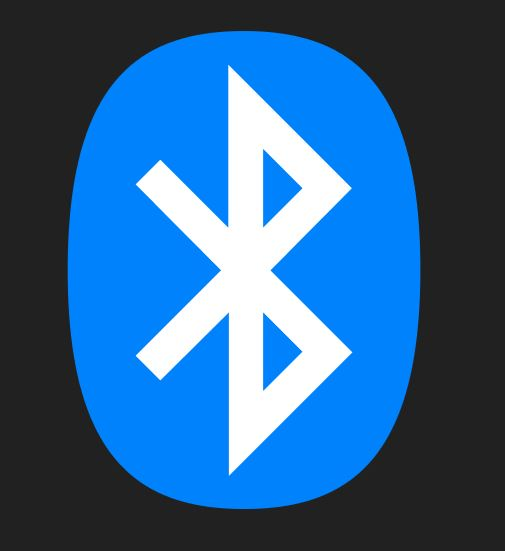
\includegraphics[width=0.55\linewidth]{images/Bluetooth.jpg}
            \caption{ لوگوی Bluetooth }
            \label{fig:h}
        \end{figure}
    }
    \item 
    {
        \textbf{Z-Wave} :
        Z-Wave یک پروتکل ارتباطی بی سیم است که عمدتاً برای اتوماسیون ساختمان های مسکونی و تجاری استفاده می شود. این یک شبکه مشبک است که از امواج رادیویی کم انرژی برای برقراری ارتباط از دستگاهی به دستگاه دیگر استفاده می کند و امکان کنترل بی سیم دستگاه های هوشمند خانه مانند چراغ های هوشمند، سیستم های امنیتی، ترموستات ها، سنسورها، قفل های هوشمند درب، و بازکننده های درب گاراژ را فراهم می کند. -برند و فناوری Wave متعلق به Silicon Labs است. بیش از 300 شرکت درگیر در این فناوری در اتحاد Z-Wave گرد هم آمده اند.
        \begin{figure}[H]
            \centering
            
\includegraphics[width=0.55\linewidth]{images/ZWave.svg.png}
            \caption{ لوگوی Z-Wave }
            \label{fig:h}
        \end{figure}
    }
    \item 
    {
        \textbf{Wi-Fi} :
        Wi-Fi خانواده ای از پروتکل های شبکه بی سیم بر اساس خانواده استانداردهای IEEE 802.11 است که معمولاً برای شبکه محلی دستگاه ها و دسترسی به اینترنت استفاده می شود و به دستگاه های دیجیتالی نزدیک اجازه می دهد تا داده ها را با امواج رادیویی مبادله کنند. اینها پرکاربردترین شبکه های کامپیوتری در جهان هستند که در سطح جهانی در شبکه های خانگی و اداری کوچک برای اتصال دستگاه ها به یکدیگر و به یک روتر بی سیم برای اتصال آنها به اینترنت و در نقاط دسترسی بی سیم در مکان های عمومی مانند کافی شاپ ها، هتل ها، کتابخانه‌ها و فرودگاه‌ها برای ارائه اتصال اینترنت به بازدیدکنندگان برای دستگاه‌های تلفن همراهشان
        استفاده می شوند.
        \begin{figure}[H]
            \centering
            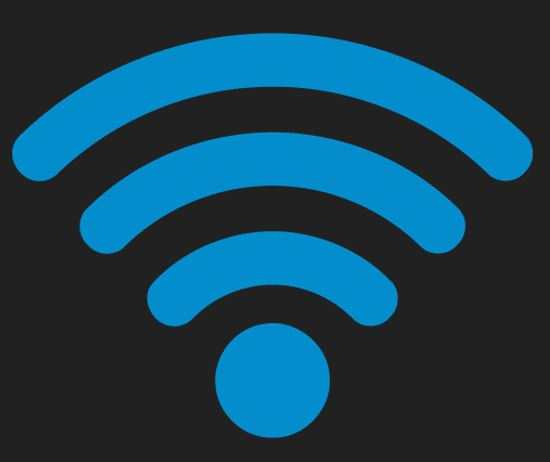
\includegraphics[width=0.6\linewidth]{images/WiFi.jpg}
            \caption{ لوگوی Wi-Fi }
            \label{fig:h}
        \end{figure}
    }
    \item 
    {
        \textbf{LoRaWAN} :
        پروتکل LoRaWAN یک پروتکل ارتباطی شبکه گسترده کم مصرف (LPWAN) است که روی LoRa کار می کند. مشخصات LoRaWAN باز است بنابراین هر کسی می تواند یک شبکه LoRa را راه اندازی و راه اندازی کند. LoRa یک فناوری فرکانس صوتی بی سیم است که در یک طیف فرکانس رادیویی بدون مجوز کار می کند.
        \begin{figure}[H]
            \centering
            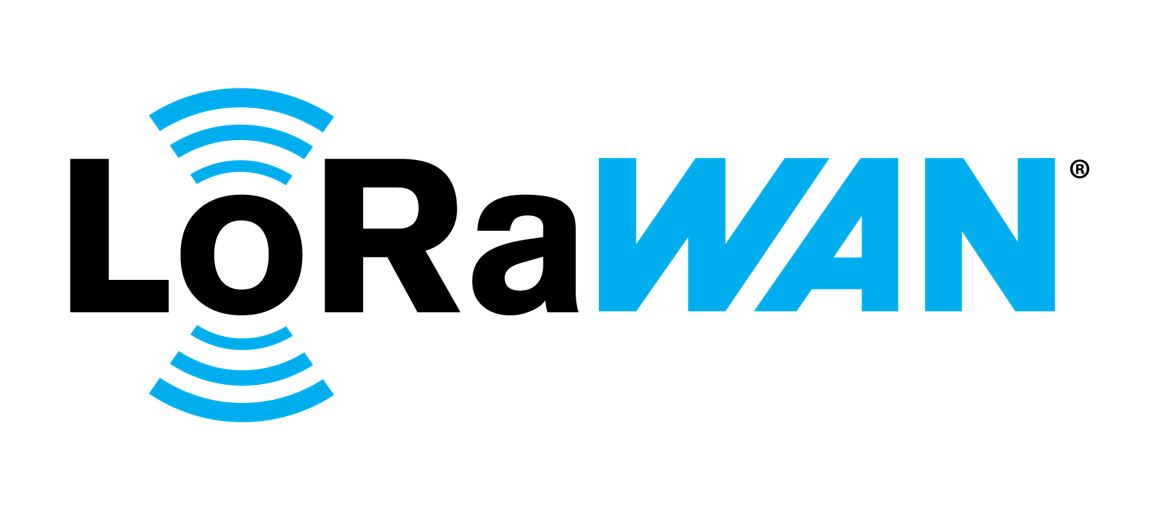
\includegraphics[width=1\linewidth]{images/LoRaWAN.jpg}
            \caption{ لوگوی LoRaWAN }
            \label{fig:h}
        \end{figure}
    }   

\end{itemize}


\subsection{مقایسه Zigbee با پروتکل های بی سیم دیگر}


\begin{itemize}

    \item 
    {
        \textbf{Bluetooth} :
        بلوتوث یک پروتکل بی سیم کوتاه برد است که معمولا برای اتصال دستگاه هایی مانند گوشی های هوشمند و هدفون استفاده می شود. بلوتوث انرژی بیشتری نسبت به ZigBee مصرف می کند و برای استقرار در مقیاس بزرگ طراحی نشده است. بلوتوث همچنین دارای تعداد محدودی دستگاه است که می توانند به شبکه متصل شوند.
    }
    \item 
    {
        \textbf{Z-Wave} :
        Z-Wave یک پروتکل بی سیم است که شبیه ZigBee است و برای برنامه های اتوماسیون خانگی طراحی شده است. Z-Wave در فرکانس متفاوتی نسبت به ZigBee کار می کند و تعداد دستگاه های کمتری را نسبت به ZigBee پشتیبانی می کند. Z-Wave همچنین برد کوتاه تری نسبت به ZigBee دارد.
    }
    \item 
    {
        \textbf{Wi-Fi} :
        Wi-Fi یک پروتکل بی سیم پرسرعت است که معمولاً برای اتصال به اینترنت استفاده می شود. 
        برخلاف ZigBee
        ،
        Wi-Fi برای برنامه های کم مصرف طراحی نشده است و انرژی بسیار بیشتری نسبت به ZigBee مصرف می کند. Wi-Fi همچنین برد کوتاه تری دارد و از شبکه مش پشتیبانی نمی کند.
    }
    \item 
    {
        \textbf{LoRaWAN} :
        LoRaWAN یک پروتکل بی سیم است که برای ارتباطات دوربرد در برنامه های کاربردی اینترنت اشیا کم مصرف طراحی شده است. 
        برخلاف ZigBee
        ،
        LoRaWAN در باندهای فرکانسی دارای مجوز عمل می کند و از محدوده بزرگتری نسبت به ZigBee پشتیبانی می کند. با این حال، LoRaWAN نرخ داده کمتری نسبت به ZigBee دارد و از شبکه مش پشتیبانی نمی کند.
    }   

\end{itemize}

% % \begin{frame}{OBJECTIVE}
% \begin{table}[h!]
%     \centering
%     % \begin{tabular}{| c | c | c | c |} 
%     % \begin{tabular}{|p{3cm}|p{3cm}|p{3cm}|p{3cm}|}
%     \begin{tabular}{p{0.15\linewidth} | p{0.20\linewidth} | p{0.2\linewidth} | p{0.20\linewidth}}
%         % Overfull \hbox (269.75974pt too wide) in paragraph at lines 100--123
        
%         \hline
%         % P(Y) & x=4 & x=3 & x=2 & x=1 & Y/X \\ [0.5ex] 
%         Wi-Fi & Bluetooth & Zigbee & Feature \\ % [0.5ex] 
%         \hline
%         2.4 GHz, 5 GHz & 2.4 GHz & 2.4 GHz, 868 MHz, 915 MHz & Frequency \\ % [0.5ex] 
%         \hline
%         Up to 100 meters (outdoor) & Up to 100 meters (outdoor) & Up to 100 meters (outdoor) & Range \\ % [0.5ex] 
%         \hline
%         Up to 6.9 Gbps & 1-3 Mbps & 20-250 Kbps & Data Rate \\
%         \hline
%         High power consumption & Moderate power consumption & Low power consumption & Power Consumption \\  % [0.5ex] 
%         \hline
%         WPA2 and other security standards & Built-in security & Built-in security & Security \\ % [0.5ex] 
%         \hline
%     \end{tabular}
%     % \caption{سلام}
%     % \label{1}
% \end{table}
% % \end{frame}


\subsection{مقایسه ZigBee با Bluetooth و Wi-Fi}
با توجه به اینکه دو پروتکل 
Bluetooth و Wi-Fi
بسیار شناخته شده و معروف هستند و کاربرد های بسیاری دارند در زیر به طور خاص به مقایسه آن ها با پروتکل 
ZigBee
می پردازیم. در این مقایسه به موارد زیر توجه می کنیم:
\begin{itemize}
    \item 
    {
        \textbf{مصرف انرژی} :
        مصرف انرژی در پروتکل 
        ZigBee
        بسیار کمتر از 
        Bluetooth
        و 
        Wi-Fi
        است. این موضوع باعث می شود که پروتکل 
        ZigBee
        برای برنامه های کم مصرف مناسب باشد.
    }
    \item 
    {
        \textbf{برد} :
        برد پروتکل 
        ZigBee
        مانند پروتکل های 
        Bluetooth
        و
        Wi-Fi
        در حدود
        از 10 تا 100 متر است.
    }
    \item 
    {
        \textbf{نرخ انتقال داده} :
        نرخ انتقال داده در پروتکل 
        ZigBee
        بسیار کمتر از 
        Bluetooth
        و 
        Wi-Fi
        است. این موضوع باعث می شود که پروتکل 
        ZigBee
        برای برنامه هایی که نیاز به نرخ انتقال داده بالا دارند مناسب نباشد.
    }
    \item 
    {
        \textbf{قیمت} :
        قیمت پروتکل 
        ZigBee
        بسیار کمتر از 
        Bluetooth
        و 
        Wi-Fi
        است. این موضوع باعث می شود که پروتکل 
        ZigBee
        برای برنامه هایی که
        \lr{budget}
        کمی دارند مناسب باشد.
    }
\end{itemize}
در زیر به طور خلاصه مقایسه ای از این سه پروتکل آورده شده است.

\begin{figure}[H]
    \centering
    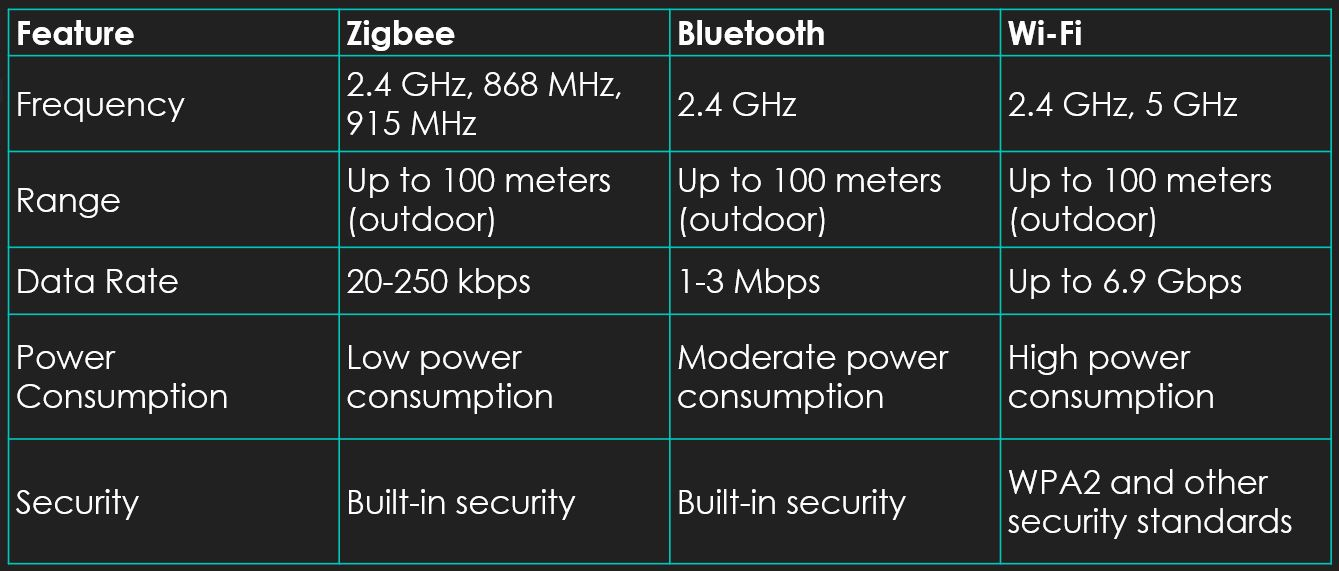
\includegraphics[width=1\linewidth]{images/comparison.jpg}
    \caption{مقایسه ZigBee با Bluetooth و Wi-Fi }
    \label{fig:h}
\end{figure}